\chapter{Symulacja dynamiczna}\label{chap:dynamic}

W tym rozdziale przedstawiono wyniki symulacji dynamicznej, która analizuje zachowanie algorytmów optymalizacyjnych w środowisku zmieniającym się w czasie. Badania obejmują sześć różnych profili mutacji grafu oraz ocenę adaptacji algorytmów do ewoluujących struktur sieciowych. Rozdział zawiera analizę zarówno mutacji syntetycznych o różnej intensywności, jak i realistycznych mechanizmów zmian topologii sieci społecznych.

\section{Założenia i konfiguracja}

Eksperymenty dynamiczne wykonano w tym samym środowisku obliczeniowym co testy statyczne. Każda symulacja obejmuje 30 kroków czasowych; w każdym kroku: (1) stosuje się mutację struktury grafu zgodnie z wybranym profilem oraz (2) przeprowadza się ponowną optymalizację dystrybucji licencji z limitem czasu \SI{45}{\second}. Analizowano dwa schematy licencyjne: Duolingo Super oraz wariant odpowiadający dominowaniu rzymskiemu. Do testów wykorzystano grafy losowe, bezskalowe oraz małego świata.

Testy przeprowadzono dla sześciu profili mutacji, przy czym każdy profil definiuje stały zestaw parametrów obowiązujący w całej symulacji. Profile obejmują trzy syntetyczne o prostej logice modyfikacji (low, med, high) oraz trzy bardziej złożone, uwzględniające mechanizmy takie jak preferencyjne przyłączanie, domykanie triad czy losowe przekształcanie krawędzi (pref\_triadic, pref\_pref, rand\_rewire).

Warianty \texttt{low}, \texttt{med} oraz \texttt{high} różnią się prawdopodobieństwami mutacji w każdym kroku symulacji (tabela~\ref{tab:dyn-mutation-levels}). W każdym kroku niezależnie decyduje się o wykonaniu danej operacji, po czym wyznacza się liczbę elementów do modyfikacji (1--3 węzłów, 1--5 krawędzi). Usunięcie węzła skutkuje usunięciem wszystkich krawędzi incydentnych z tym węzłem. Prawdopodobieństwa dobrano w celu uzyskania trzech odrębnych poziomów intensywności zmian: niskiego (modyfikacje w ~1--6\% kroków), średniego (4--18\%) oraz wysokiego (8--30\%).

\begin{table}[H]
    \centering
    \caption{Parametry intensywności mutacji w symulacji dynamicznej.}
    \label{tab:dyn-mutation-levels}
    \begin{tabular}{lcccc}
        \toprule
        \textbf{Poziom} & \textbf{Dodawanie węzłów} & \textbf{Usuwanie węzłów} & \textbf{Dodawanie krawędzi} & \textbf{Usuwanie krawędzi} \\
        \midrule
        low             & 0.02                      & 0.01                     & 0.06                        & 0.04                       \\
        med             & 0.06                      & 0.04                     & 0.18                        & 0.12                       \\
        high            & 0.12                      & 0.08                     & 0.30                        & 0.20                       \\
            \bottomrule
    \end{tabular}
\end{table}


Dodatkowo zbadano trzy bardziej realistyczne profile ewolucji sieci. Wszystkie operują na tych samych limitach liczby dodawanych/usuwanych elementów co warianty syntetyczne, różnią się jednak mechanizmem wyboru sąsiedztwa.

Wariant \texttt{pref\_triadic} łączy dwa mechanizmy typowe dla sieci społecznych: preferencyjne przyłączanie i domykanie triad. Nowe węzły dołączają do sieci, preferencyjnie łącząc się z istniejącymi węzłami o wysokim stopniu. Nowe krawędzie powstają poprzez domykanie trójkątów, tj. łączenie dwóch niepołączonych węzłów mających wspólnego sąsiada. Mechanizm ten wzmacnia lokalną strukturę klastrową sieci, co odzwierciedla tendencję do tworzenia zamkniętych grup w rzeczywistych sieciach~\cite{albert2002statistical,kamola2016dynamika}.

Wariant \texttt{pref\_pref} stosuje mechanizm preferencyjnego przyłączania zarówno przy dodawaniu nowych węzłów, jak i tworzeniu krawędzi między już istniejącymi. Oznacza to, że zarówno nowe węzły, jak i nowe krawędzie preferencyjnie łączą wierzchołki o wysokim stopniu. Takie podejście sprzyja tworzeniu centralnych węzłów o wysokim stopniu w sieci, co jest kluczową cechą topologii bezskalowych~\cite{albert2002statistical}.

Wreszcie wariant \texttt{rand\_rewire} wprowadza do sieci element losowości, inspirowany modelem Wattsa i Strogatza. Nowe węzły dołączane są w sposób losowy, bez preferencji dla popularniejszych wierzchołków. Zamiast dodawać krawędzie, model modyfikuje strukturę poprzez przełączanie: losową krawędź usuwa się, po czym jeden z jej końców łączy się z innym losowo wybranym węzłem. Proces ten prowadzi do powstawania połączeń długozasięgowych i zmniejsza regularność struktury grafu~\cite{watts1998collective}.



\section{Algorytm zachłanny}

W tym wariancie algorytm zachłanny w każdym kroku symulacji buduje rozwiązanie całkowicie od zera, ignorując poprzednie wyniki optymalizacji. Stanowi to dolne ograniczenie narzutu czasowego dla metod konstruktywnych oraz punkt odniesienia jakościowy, względem którego porównywane są bardziej zaawansowane metaheurystyki wykorzystujące rozwiązania z poprzednich kroków jako punkt startowy dla dalszej optymalizacji.

\subsection{Zestawienie dla wszystkich mutacji}
Tabela~\ref{tab:greedy-cold-summary} zestawia średni koszt na węzeł i średni czas wykonania algorytmu na krok symulacji dla sześciu badanych profili mutacji: trzech syntetycznych oraz trzech realistycznych. Wszystkie czasy mieszczą się w przedziale od \SI{0.5}{\milli\second} do \SI{1.8}{\milli\second} na krok, a średni koszt na węzeł oscyluje wokół 0.46 do 0.48.

\begin{table}[H]
    \centering
    \caption{Algorytm zachłanny: średni koszt na węzeł oraz średni czas na krok dla wszystkich wariantów mutacji.}
    \label{tab:greedy-cold-summary}
    \begin{tabular}{lcc}
        \toprule
        \textbf{Metoda mutacji} & \textbf{Koszt/węzeł (mean)} & \textbf{Średni czas [s]} \\
        \midrule
        high                    & 0.48009                     & 0.00159                  \\
        low                     & 0.47983                     & 0.00165                  \\
        med                     & 0.47491                     & 0.00181                  \\
        pref\_pref              & 0.46371                     & 0.00083                  \\
        pref\_triadic           & 0.46787                     & 0.00053                  \\
        rand\_rewire            & 0.47556                     & 0.00083                  \\
        \bottomrule
    \end{tabular}
\end{table}

Algorytm zachłanny charakteryzuje się krótkim czasem wykonania, co uzasadnia jego użycie jako czasowego punktu odniesienia w środowisku dynamicznym. Warianty realistyczne sprzyjają nieco niższym kosztom: \texttt{pref\_pref} osiąga najniższy średni koszt (0.464), a \texttt{pref\_triadic} jest jednocześnie najszybszy (\SI{0.00053}{\s}). Wariant \texttt{rand\_rewire} jest trudniejszy (0.476), ale pozostaje bardzo szybki czasowo.

Różnice kosztu dla mutacji syntetycznych są niewielkie (0.475--0.480), natomiast czasy są wyższe niż w profilach realistycznych, szczególnie dla \texttt{med/high}. Wskazuje to, że lokalne, realistyczne przekształcenia są mniej kosztowne obliczeniowo do przetwarzania. Czasy dla \texttt{pref\_pref} wynoszą średnio \SI{0.00083}{\s}, a dla \texttt{pref\_triadic} \SI{0.00053}{\s}, co potwierdza ich przewagę czasową nad mutacjami syntetycznymi (\SI{0.00159}{\s} dla \texttt{high}).

\section{Analiza mutacji syntetycznych}

Ta sekcja prezentuje szczegółową analizę zachowania algorytmów przy trzech poziomach intensywności mutacji syntetycznych: low, med oraz high. Badania skupiają się na ocenie adaptacyjności metaheurystyk do zmian o różnej skali oraz analizie kompromisu między jakością rozwiązania a czasem wykonania.

\subsection{Metaheurystyki}

Tabela~\ref{tab:dyn-synth-warm} przedstawia zbiorcze wyniki dla różnych metod mutacji. Średni koszt na węzeł jest bardzo zbliżony dla wszystkich poziomów intensywności, z jedynie nieznacznym wzrostem dla wariantu \texttt{high}. Sugeruje to, że algorytmy są w stanie skutecznie adaptować się do zmian w topologii sieci.

Średni czas wykonania rośnie wraz z intensywnością mutacji. Wariant \texttt{low} jest najszybszy, podczas gdy \texttt{high} wymaga najwięcej czasu na ponowne zbilansowanie. Jest to naturalna konsekwencja faktu, że większa liczba modyfikacji grafu (dodawanie/usuwanie węzłów i krawędzi) stanowi większe wyzwanie obliczeniowe dla algorytmów optymalizacyjnych. Różnice czasów pozostają umiarkowane, co wskazuje na korzystną skalowalność zastosowanych metod.

\begin{table}[H]
    \centering
    \caption{Wyniki dla różnych metod mutacji.}
    \label{tab:dyn-synth-warm}
    \begin{tabular}{lcc}
        \toprule
        \textbf{Metoda mutacji} & \textbf{Średni koszt} & \textbf{Średni czas [s]} \\
        \midrule
        high                    & 0.4893                & 3.169                    \\
        med                     & 0.4850                & 3.075                    \\
        low                     & 0.4852                & 2.878                    \\
        \bottomrule
    \end{tabular}
\end{table}

\subsection{Profil kosztu i czasu w czasie}
Jako przykład ewolucji kosztu i czasu w krokach symulacji wybrano algorytm genetyczny. Rysunki~\ref{fig:dyn-synth-genetic-cost} i~\ref{fig:dyn-synth-genetic-time} przedstawiają odpowiednio przebieg kosztu na węzeł oraz czasu wykonania w zależności od kroku symulacji dla różnych poziomów intensywności mutacji.

Dla wariantu \texttt{high} można zaobserwować niewielkie, lecz zauważalne wahania średniego kosztu na węzeł, które nie są tak widoczne w przypadku wariantów \texttt{low} i \texttt{med}. W zakresie czasów wykonania dla wszystkich trzech wariantów występują porównywalne wahania w trakcie symulacji.

\begin{figure}[H]
    \centering
    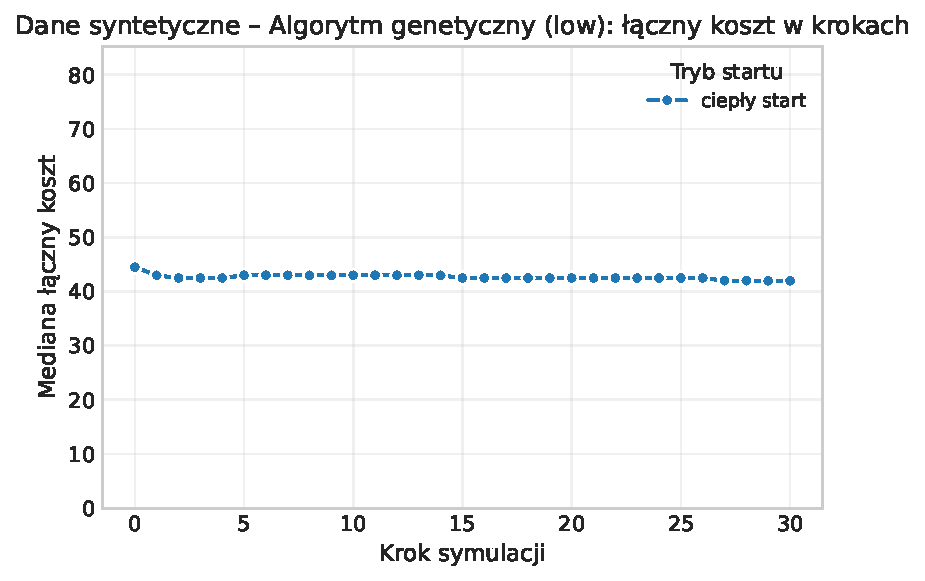
\includegraphics[width=0.32\linewidth]{assets/figures/dynamic/synthetic/synthetic_algorytm_genetyczny_cost_over_steps_low.pdf}
    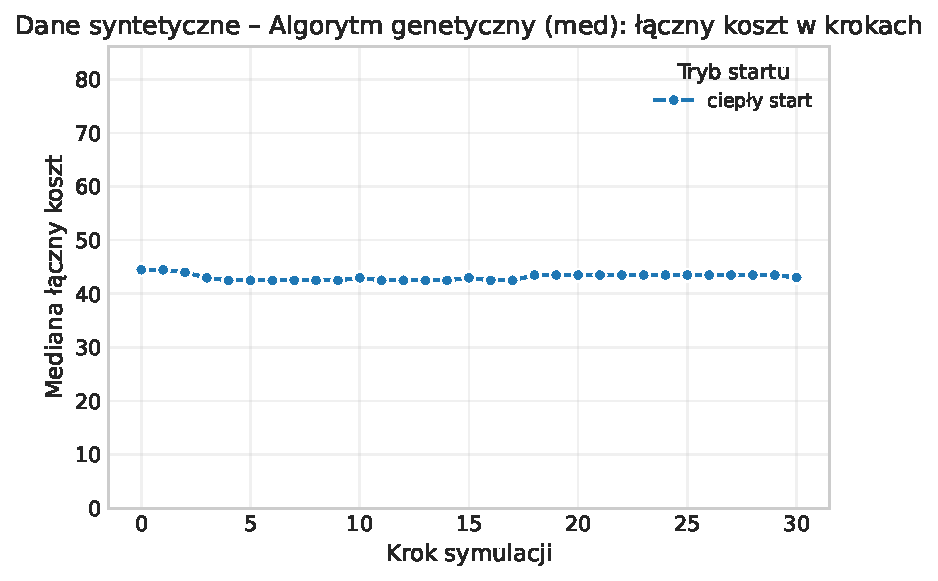
\includegraphics[width=0.32\linewidth]{assets/figures/dynamic/synthetic/synthetic_algorytm_genetyczny_cost_over_steps_med.pdf}
    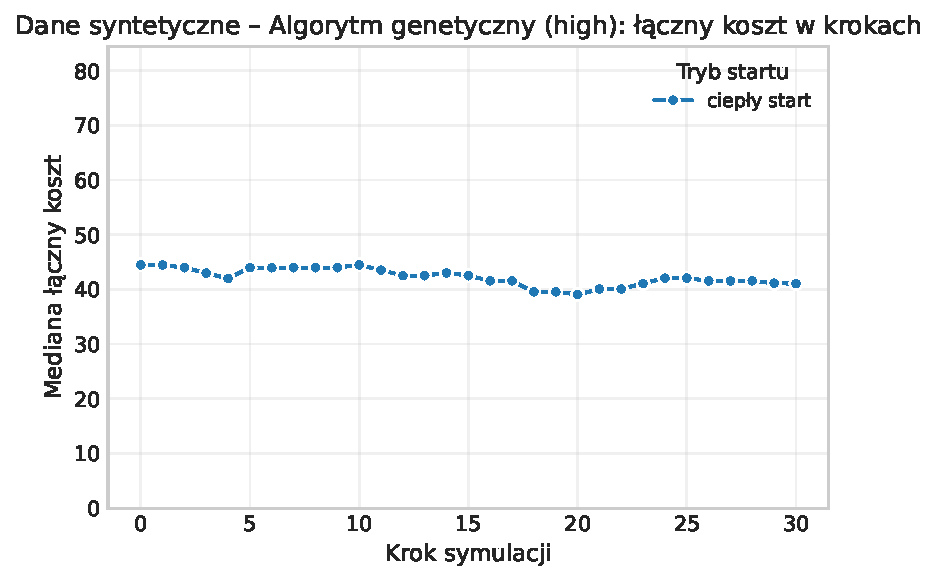
\includegraphics[width=0.32\linewidth]{assets/figures/dynamic/synthetic/synthetic_algorytm_genetyczny_cost_over_steps_high.pdf}
    \caption{Algorytm genetyczny -- koszt na węzeł w kolejnych krokach symulacji (warianty low/med/high).}
    \label{fig:dyn-synth-genetic-cost}
\end{figure}

\begin{figure}[H]
    \centering
    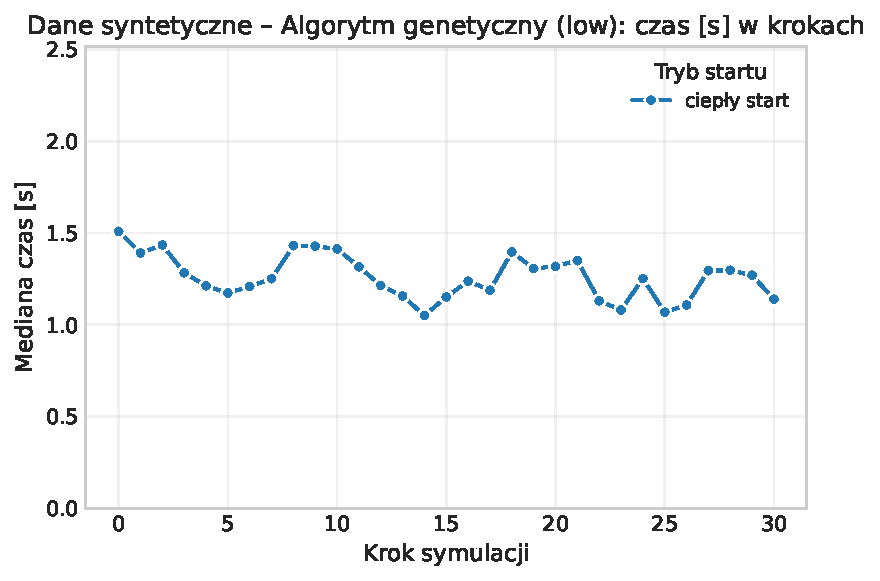
\includegraphics[width=0.32\linewidth]{assets/figures/dynamic/synthetic/synthetic_algorytm_genetyczny_time_over_steps_low.pdf}
    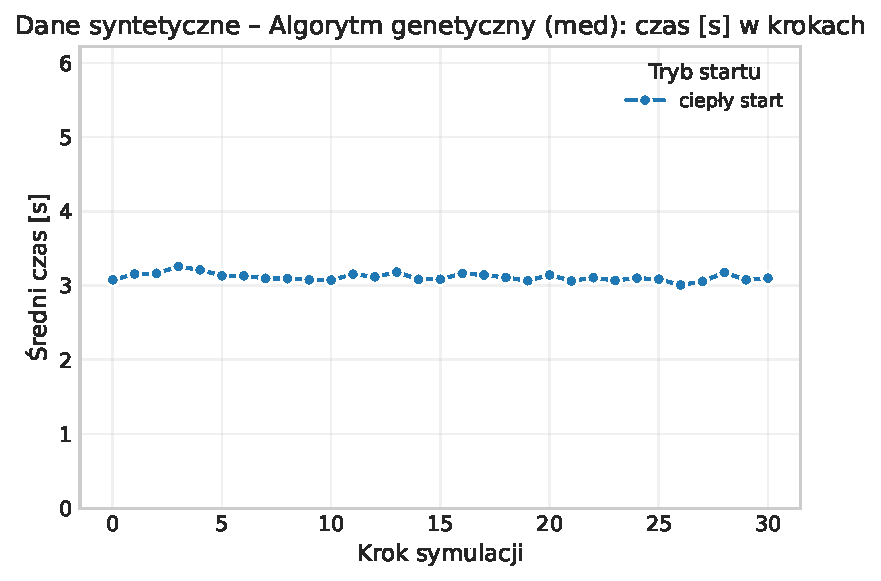
\includegraphics[width=0.32\linewidth]{assets/figures/dynamic/synthetic/synthetic_algorytm_genetyczny_time_over_steps_med.pdf}
    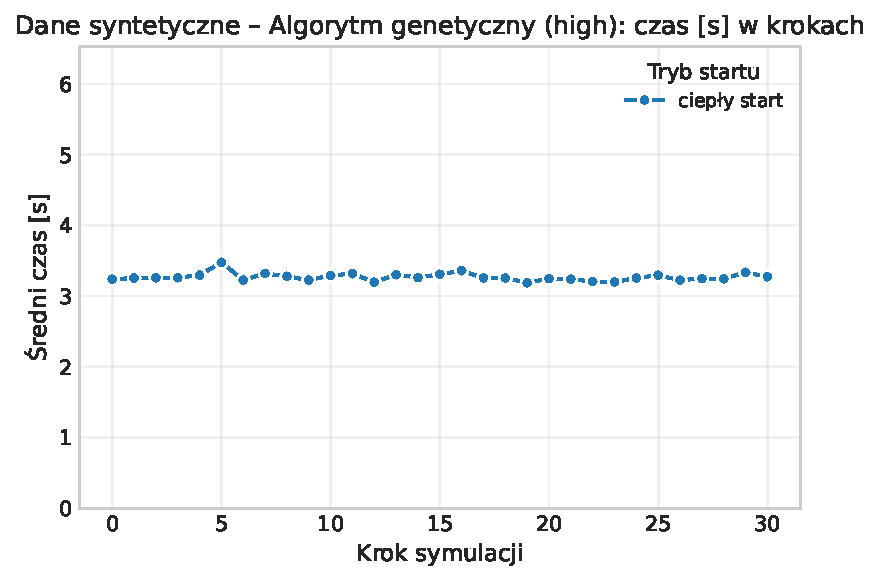
\includegraphics[width=0.32\linewidth]{assets/figures/dynamic/synthetic/synthetic_algorytm_genetyczny_time_over_steps_high.pdf}
    \caption{Algorytm genetyczny -- czas wykonania w kolejnych krokach symulacji (warianty low/med/high).}
    \label{fig:dyn-synth-genetic-time}
\end{figure}

\section{Analiza mutacji realistycznych}
Tabela~\ref{tab:dyn-real-warm} przedstawia zbiorcze wyniki dla opracowanych scenariuszy realistycznych. Wariant \texttt{pref\_triadic} wyróżnia się najkrótszym średnim czasem wykonania (poniżej \SI{1}{\second}), przy zachowaniu kosztu na poziomie zbliżonym do wariantu \texttt{pref\_pref}. Z kolei scenariusz \texttt{rand\_rewire} okazał się najbardziej wymagający dla algorytmów -- charakteryzuje się jednocześnie najwyższym średnim kosztem i najdłuższym czasem przetwarzania. Przyczyną jest losowe przełączanie krawędzi, które zaburza lokalną klastrowość, zwiększa entropię topologii i utrudnia użycie poprzedniego rozwiązania jako punktu startowego. W efekcie optymalizacja wymaga więcej iteracji, a uzyskana jakość jest gorsza.


\begin{table}[H]
    \centering
    \caption{Wyniki dla różnych metod mutacji w scenariuszach realistycznych.}
    \label{tab:dyn-real-warm}
    \begin{tabular}{lccc}
        \toprule
        \textbf{Metoda mutacji} & \textbf{Średni koszt całkowity} & \textbf{Koszt/węzeł (mean)} & \textbf{Średni czas [s]} \\
        \midrule
        pref\_pref              & 113.34                          & 0.4764                      & 1.6774                   \\
        pref\_triadic           & 70.08                           & 0.4764                      & 0.8619                   \\
        rand\_rewire            & 116.83                          & 0.4917                      & 1.8421                   \\
        \bottomrule
    \end{tabular}
\end{table}

\subsection{Wybrane algorytmy i metody mutacji}
W celu zilustrowania zachowania różnych algorytmów optymalizacyjnych w środowisku dynamicznym, wybrano reprezentatywne pary algorytmów i metod mutacji. Zestawienie obejmuje algorytmy o różnej złożoności obliczeniowej, od prostych heurystyk po metaheurystyki, testowane na wybranych profilach mutacji realistycznych i syntetycznych. Dobór przedstawia spektrum możliwych rozwiązań, od szybkich metod przybliżonych po dokładne, ale czasochłonne podejścia optymalizacyjne.

\begin{table}[H]
    \centering
    \caption{Wybrane pary algorytmów i metod mutacji.}
    \label{tab:dyn-synth-selected-best}
    \begin{tabular}{llccc}
        \toprule
        \textbf{Algorytm}     & \textbf{Metoda} & \textbf{Liczba kroków} & \textbf{Koszt/węzeł} & \textbf{Śr. czas [s]} \\
        \midrule
        Algorytm ILP          & pref\_triadic   & 434                    & 0.362                & 1.525                 \\
        Algorytm ILP          & rand\_rewire    & 496                    & 0.390                & 2.553                 \\
        Algorytm genetyczny   & pref\_triadic   & 744                    & 0.409                & 0.615                 \\
        Algorytm genetyczny   & pref\_pref      & 930                    & 0.414                & 1.134                 \\
        Przeszukiwanie tabu   & pref\_triadic   & 744                    & 0.413                & 1.470                 \\
        Przeszukiwanie tabu   & rand\_rewire    & 930                    & 0.445                & 2.581                 \\
        Algorytm mrówkowy     & pref\_pref      & 899                    & 0.417                & 6.906                 \\
        Algorytm mrówkowy     & pref\_triadic   & 744                    & 0.424                & 3.002                 \\
        Wyżarzanie symulowane & pref\_triadic   & 744                    & 0.460                & 0.555                 \\
        Algorytm zachłanny    & pref\_pref      & 930                    & 0.464                & 0.001                 \\
        Zbiór dominujący      & pref\_triadic   & 744                    & 0.457                & 0.005                 \\
        Algorytm losowy       & pref\_pref      & 930                    & 0.754                & 0.001                 \\
        \bottomrule
    \end{tabular}
\end{table}

Algorytm ILP osiąga najniższe koszty, lecz wymaga około \SI{1.5}-\SI{2.6}{\second} na krok. Algorytm genetyczny dobrze sprawdza się przy zmianach klastrowych (\texttt{pref\_triadic}), oferując niski koszt i czas około \SI{0.6}{\second}. Przy wariancie \texttt{pref\_pref} jest wolniejszy (\SI{1.1}{\second}), ale zachowuje dobrą jakość. Z kolei wyżarzanie symulowane jest szybkie (około \SI{0.5}{\second}) i stabilne, ale jakościowo ustępuje bardziej zaawansowanym metodom.

Przeszukiwanie tabu korzysta z lokalności zmian, osiągając sensowny koszt i czas około \SI{1.5}{\second} przy \texttt{pref\_triadic}. Jednak przy mutacjach losowych (\texttt{rand\_rewire}) czas wzrasta do około \SI{2.6}{\second}, a koszt również rośnie. Algorytm mrówkowy zapewnia bardzo dobrą jakość przy \texttt{pref\_pref}, ale działa najwolniej (prawie \SI{7}{\second}). Przejście na \texttt{pref\_triadic} ponad dwukrotnie przyspiesza jego działanie kosztem niewielkiego pogorszenia jakości.

Szybkie heurystyki, takie jak algorytm zachłanny (≈\SI{1}{\milli\second}) i zbiór dominujący (≈\SI{5}{\milli\second}), są efektywne czasowo. Zbiór dominujący zwykle osiąga niższy koszt niż zachłanny, co czyni go zasadnym wyborem przy ograniczeniach czasowych. Mutacje klastrowe (\texttt{pref\_triadic}, \texttt{pref\_pref}) pomagają wszystkim algorytmom utrzymać niski średni koszt licencji liczony na jeden węzeł i krótszy czas. Natomiast \texttt{rand\_rewire} zwiększa zarówno koszt, jak i czas.


\subsection{Ewolucja kosztów w czasie}
Pełne przebiegi dla algorytmu genetycznego pokazano na rys.~\ref{fig:dyn-real-genetic-cost}--\ref{fig:dyn-real-genetic-time}. Łączenie preferencyjnego przyłączania z triadycznym domykaniem sprzyja utrzymaniu najniższych kosztów, natomiast wariant z losowym przełączaniem krawędzi prowadzi do wolniejszej stabilizacji. Analizując koszt na węzeł na rys. \ref{fig:dyn-real-genetic-cost}, można zauważyć, że dla każdego z typów mutacji przebiega on podobnie, oscylując wokół zbliżonego poziomu.

Z kolei, patrząc na czas wykonania na rys. \ref{fig:dyn-real-genetic-time}, widać, że dla wariantu \texttt{rand\_rewire} występują największe wahania, co sugeruje większą niestabilność procesu optymalizacji. Warianty \texttt{pref\_triadic} i \texttt{pref\_pref} charakteryzują się bardziej stabilnym czasem wykonania.

\begin{figure}[H]
    \centering
    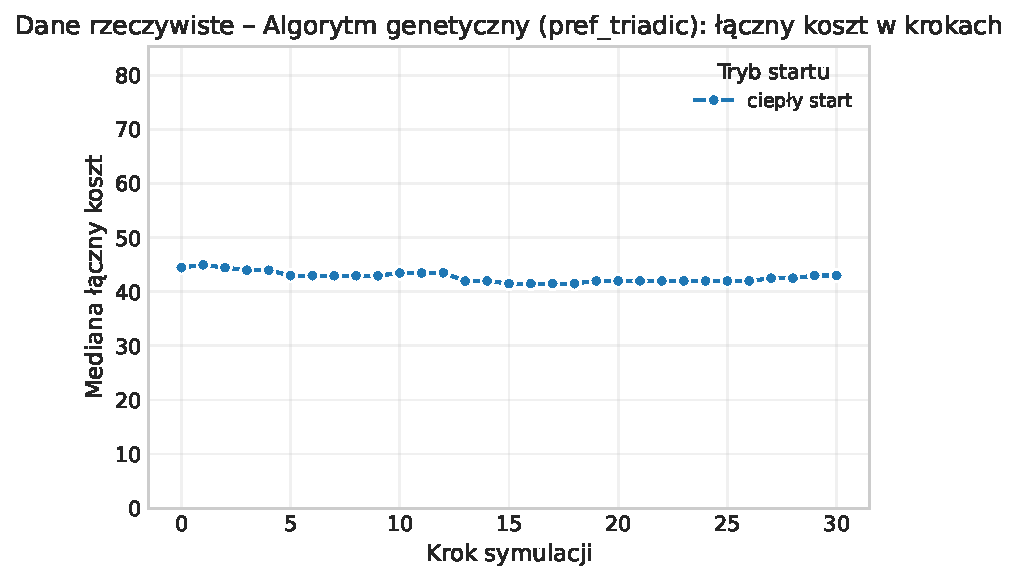
\includegraphics[width=0.32\linewidth]{assets/figures/dynamic/real/real_algorytm_genetyczny_cost_over_steps_pref_triadic.pdf}
    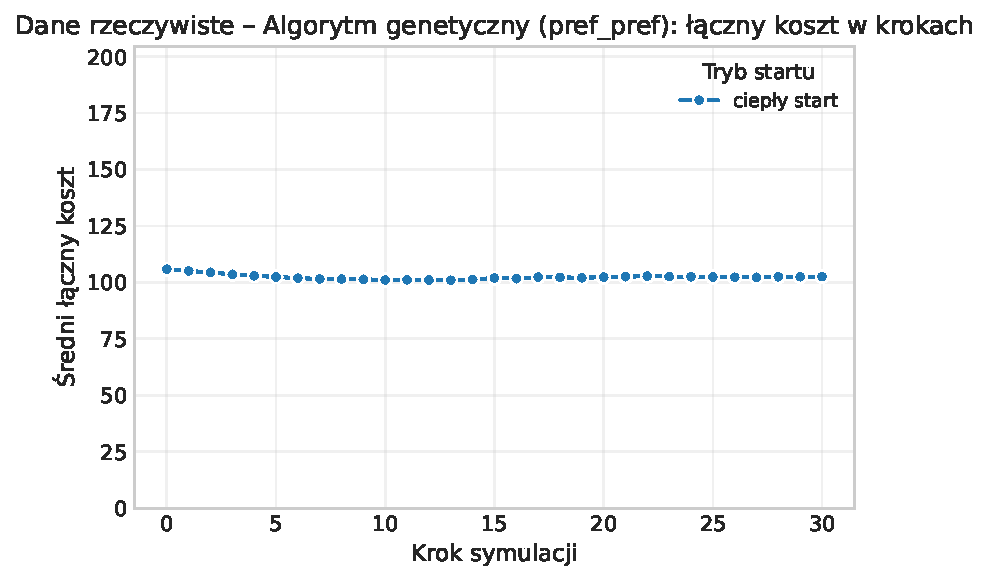
\includegraphics[width=0.32\linewidth]{assets/figures/dynamic/real/real_algorytm_genetyczny_cost_over_steps_pref_pref.pdf}
    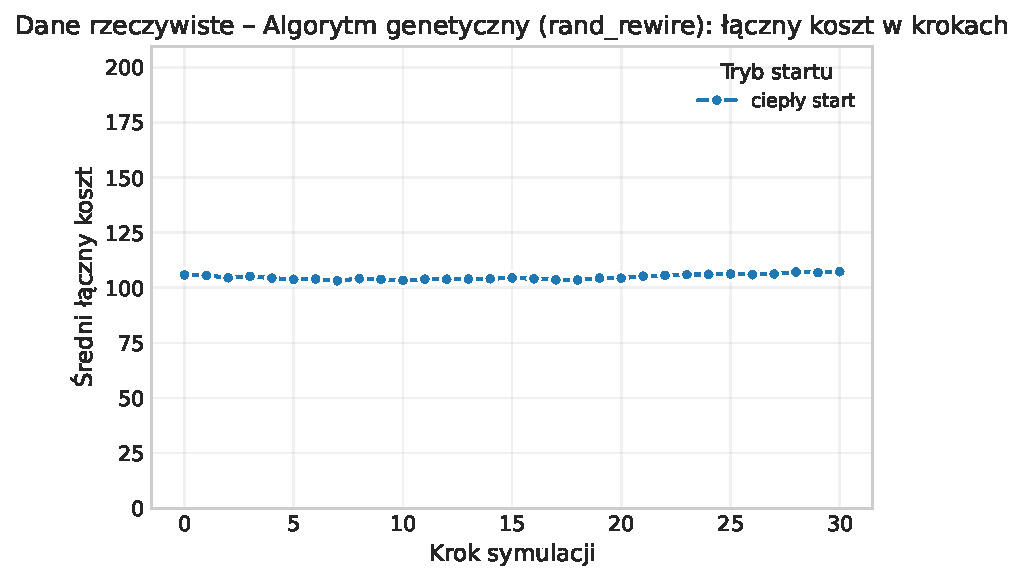
\includegraphics[width=0.32\linewidth]{assets/figures/dynamic/real/real_algorytm_genetyczny_cost_over_steps_rand_rewire.pdf}
    \caption{Algorytm genetyczny -- koszt na węzeł w wariantach realistycznych.}
    \label{fig:dyn-real-genetic-cost}
\end{figure}

\begin{figure}[H]
    \centering
    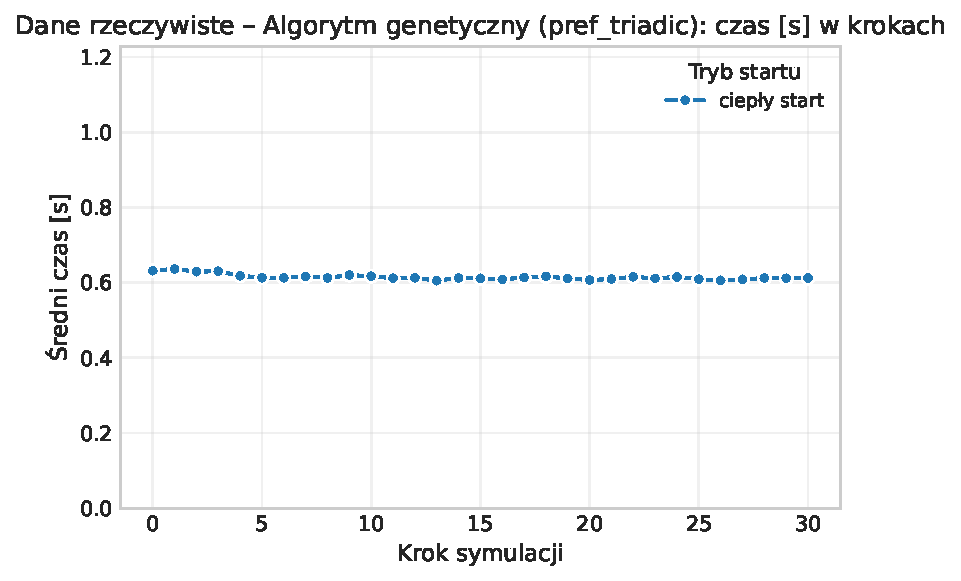
\includegraphics[width=0.32\linewidth]{assets/figures/dynamic/real/real_algorytm_genetyczny_time_over_steps_pref_triadic.pdf}
    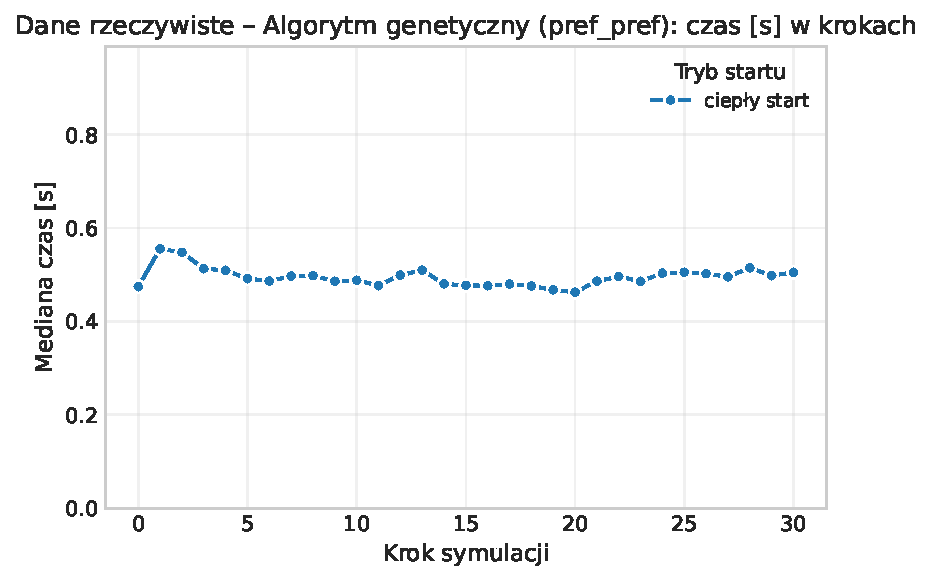
\includegraphics[width=0.32\linewidth]{assets/figures/dynamic/real/real_algorytm_genetyczny_time_over_steps_pref_pref.pdf}
    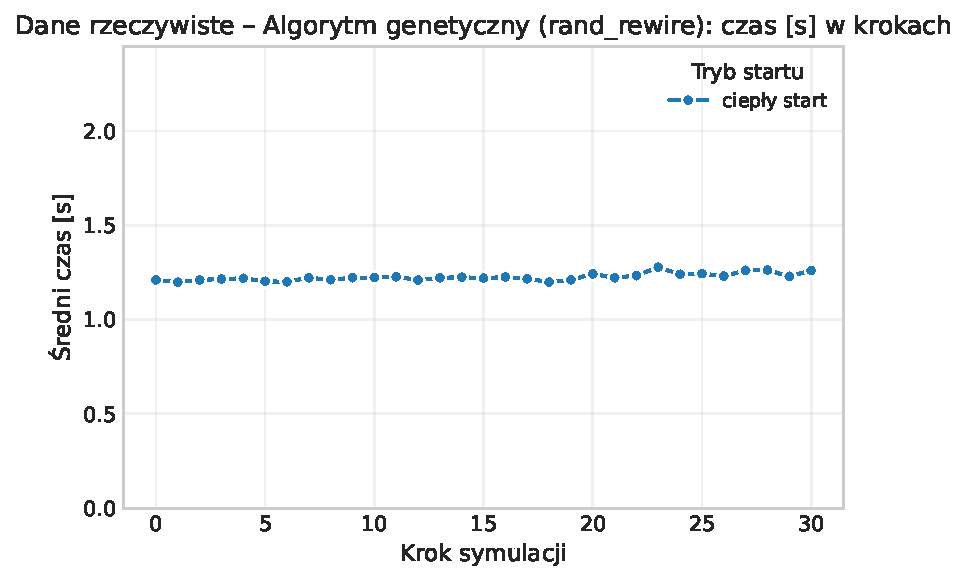
\includegraphics[width=0.32\linewidth]{assets/figures/dynamic/real/real_algorytm_genetyczny_time_over_steps_rand_rewire.pdf}
    \caption{Algorytm genetyczny -- czas wykonania w wariantach realistycznych.}
    \label{fig:dyn-real-genetic-time}
\end{figure}

\section{Wnioski}

Przeprowadzona analiza dynamiczna wykazała, że dobór algorytmu optymalizacyjnego w środowisku dynamicznym powinien uwzględniać zarówno profil zmian topologii sieci, jak i dostępny budżet czasowy. Badania obejmujące sześć wariantów mutacji (trzy syntetyczne oraz trzy realistyczne) na różnych typach grafów pozwoliły na sformułowanie kluczowych wniosków dotyczących adaptacji algorytmów do ewoluujących struktur sieciowych.

Mutacje realistyczne, takie jak \texttt{pref\_triadic} oraz \texttt{pref\_pref}, były mniej wymagające obliczeniowo do obsłużenia w porównaniu z wariantami syntetycznymi o wysokiej intensywności. Mechanizmy preferencyjnego przyłączania oraz domykania trójkątów sprzyjają wzmacnianiu klastrowości i tworzeniu hubów, co zmniejsza efektywny rozmiar problemu pokrycia. W rezultacie algorytmy osiągały niższe koszty (0.470--0.475 w porównaniu do 0.485--0.489) oraz krótsze czasy wykonania (0.9--1.7 s w porównaniu do 2.9--3.2 s). Z kolei mutacje typu \texttt{rand\_rewire} zwiększały entropię topologii poprzez zrywanie lokalnych połączeń, co prowadziło do najgorszych wyników zarówno pod względem kosztu (0.486), jak i czasu (1.9 s).

Algorytmy wykazywały różną odporność na poszczególne typy zmian w zależności od mechanizmu wykorzystania poprzedniego rozwiązania. Algorytm ILP zapewniał najwyższą jakość (koszt 0.362--0.390), lecz wymagał znacznego czasu na ponowne rozwiązanie zmodyfikowanych ograniczeń. Algorytm genetyczny dobrze radził sobie przy zmianach klastrowych, oferując korzystny kompromis między jakością a czasem (koszt 0.409 przy czasie 0.615 s dla \texttt{pref\_triadic}), jednak jego efektywność spadała w przypadku mutacji destrukcyjnych. Przeszukiwanie tabu, jako metoda intensywnie lokalna, sprawdzało się przy zmianach o ograniczonym zasięgu, lecz przy mutacjach o większej skali wymagało rozszerzenia promienia poszukiwań, co wydłużało czas działania do około \SI{6.5}{\second}.

Szybkie heurystyki, takie jak algorytm zachłanny oraz zbiór dominujący, zachowywały swoją użyteczność również w środowisku dynamicznym, oferując czasy wykonania poniżej \SI{5}{\milli\second} przy kosztach porównywalnych z bardziej złożonymi metodami. Algorytm zachłanny osiągał stabilny czas w zakresie od \SI{0.5}{\milli\second} do \SI{1.8}{\milli\second} przy koszcie 0.464--0.480, natomiast zbiór dominujący zapewniał nieco niższy koszt przy czasie około \SI{5}{\milli\second}.

Wyniki badań wskazują na konieczność adaptacyjnego doboru strategii optymalizacyjnej w zależności od obserwowanego profilu zmian. Przy zmianach o charakterze klastrowym zaleca się stosowanie metaheurystyk z mechanizmami naprawy poprzedniego rozwiązania. W przypadku zmian chaotycznych konieczne może być głębsze odświeżenie rozwiązania lub zaakceptowanie wyższego kosztu w zamian za stabilność czasową. Gdy czas jest krytycznym ograniczeniem, szybkie heurystyki są preferowane ze względu na przewidywalną wydajność niezależnie od typu mutacji.

Najlepszy kompromis oferują metaheurystyki łączące konstrukcję z wykorzystaniem poprzedniego rozwiązania i lokalne naprawy, adaptowane do intensywności zmian między krokami.
